\documentclass[SDSUThesis.tex]{subfiles} 
\begin{document}

\newpage
\pagenumbering{arabic}
\setcounter{tocdepth}{2}

% see this for  guidance https://www.cs.purdue.edu/homes/dec/essay.dissertation.html
\section{INTRODUCTION}

Software is becoming a vital part of companies. In 2011 Marc Andreessen, co-founder of the venture capital firm Andreessen-Horowitz,
famously claimed, ``Software is Eating The World'' \cite{Andreessen2001}. His argument was for the ever increasing importance of software
in all organizations big and small regardless of the industry.  With this important declaration, the production of new software is
going to be critical.  Just as important will be the effective measurement of how this software is produced.  

The goal of this work is to provide a basis of what data should be collected by a software development organization, and how that data
should be used to formulate a single number representing the software development score of an organization. A framework to 
achieve the score will be presented.  The  score
is not to be comparative between organizations, but to rather form a historical baseline for a specific organization.  Also, a software
system to collect, calculate, and report the score will be presented.

\subsection{BACKGROUND}

Throughout the history of software development, many values have been collected and used to measure the effectiveness of software development. 
Many metrics have been used in the past and are still being used.  A metric can be defined as the science of indirect measurement.
The following are some examples of metrics that can be collected about source code:
\begin{itemize}
\item SLOC - The number of Source Lines of Code 
\item NOM - The Number of Methods per class
\item Complexity - A numerical measure of the code complexity, some common examples are McCabe \cite{McCabe1976} and Halstead \cite{Halstead1977}
\item Design - The amount of coupling and cohesion present in the software code
\item Source Code Analysis - Tools that determine whether code adheres to specified set of rules. Common examples are PMD and findbugs.
\end{itemize}

However, the metrics on source code only explain part of the software development lifecycle.  
Most of the effort has been placed on measuring just the computer code and not the entire organization.  Software
development involves more than just source code.

\subsection{CMMI}
The Capability Maturity Model Integration (CMMI) is one of the most widely acknowledged models for process 
improvement in software development.  CMMI offers a generic guideline and appraisal program for process 
improvement.  It was created and is administered by the Software Engineering Institute at
Carnegie Mellon University. While the CMMI is not specific to software development,
it is often applied in software development settings.
CMMI certification is required for many United States Government and Department of Defense contracts. 

CMMI-Dev is a modification of the CMMI specific to the development activities applied to products
and services \cite{CMMI}.  The practices covered in CMMI-Dev include project management, 
systems engineering, hardware engineering, process management, software engineering, and 
other maintenance processes.  Five maturity levels are specified, and they include the 
existence of a number of process areas.  The 5 maturity levels and the process areas are
specified as follows.

\subsubsection{CMMI MATURITY LEVEL 1 - INITIAL}
    A maturity level 1 organization consists of a adhoc and chaotic processes.  While working
    products are still produced, the results are often over budget and behind schedule.  A level
    1 organization will also have difficulties repeating a process with the same degree of 
    success.  These organizations typically rely on the heroic efforts of certain individuals. 
    
\subsubsection{CMMI MATURITY LEVEL 2 - MANAGED}
    A maturity level 2 organization has a policy for planning and executing processes.  
    The processes are controlled, monitored, reviewed, and enforced.  The practices are even
    maintained in times of stress.  The following process areas should be present at maturity
    level 2.
    \begin{description}
        \item Configuration Management (CM)
        \item Measurement and Analysis (MA)
        \item Project Monitoring and Control (PMC)
        \item Project Planning (PP)
        \item Process and Product Quality Assurance (PPQA)
        \item Requirements Management (REQM)
        \item Supplier Agreement Management (SAM)
    \end{description}

\subsubsection{CMMI MATURITY LEVEL 3 - DEFINED}
    A maturity level 3 organization has well-understood processes that are described in 
    standards, tools, procedures, and methods.  The organization has standard processes
    that are reviewed and improved over time.  The major differentiators between level 2 
    and level 3 is the existence of standards and process descriptions. 
    A level 2 organization will have
    processes that are inconsistent across projects.  A level 3 organization will tailor
    a standard process for each project.  Also, level 3 processes are described with 
    much more rigor.  In addition to the process areas found in level 2, 
    the following process areas should be present at maturity level 3.
    \begin{itemize}
        \item Decision Analysis and Resolution (DAR)
        \item Integrated Project Management (IPM)
        \item Organizational Process Definition (OPD)
        \item Organizational Process Focus (OPF)
        \item Organizational Training (OT)
        \item Product Integration (PI)
        \item Requirements Development (RD)
        \item Risk Management (RSKM)
        \item Technical Solution (TS)
        \item Validation (VAL)
        \item Verification (VER)
    \end{itemize}
    
\subsubsection{CMMI MATURITY LEVEL 4 - QUALITATIVELY MANAGED}
    A maturity level 4 organization has quantitative measures for quality and process performance. 
    The measures are based upon customer needs, end users, and process implementers.  The quality
    and process performance are understood mathematically and managed throughout the life of a project.
    Level 4 is characterized by the predictability of the process performance. In addition to
    the process areas found in level 2 and 3, the following additional process areas should be present
    at maturity level 4.
    \begin{itemize}
        \item Organizational Process Performance (OPP)
        \item Quantitative Project Management (QPM)
    \end{itemize}
\subsubsection{CMMI MATURITY LEVEL 5 - OPTIMIZING} 
    The final and pinnacle level of CMMI maturity is level 5.  A maturity level 5 organization
    continually improves processes based upon quantitative measures.  The major distinction from 
    level 4 is the constant focus on improving and managing organizational performance.  A maturity level
    5 organization has well-documented standard processes that are tracked and enforced as well as
    a focus on continual improvement of the processes based upon 
    quantitative measures.  In addition to the process areas of the previous maturity levels, maturity
    level 5 should contain the following process areas.
    \begin{itemize}
        \item Causal Analysis and Resolution (CAR)
        \item Organizational Performance Management (OPM)
    \end{itemize}

        
        \begin{figure}[here]
            \centering
            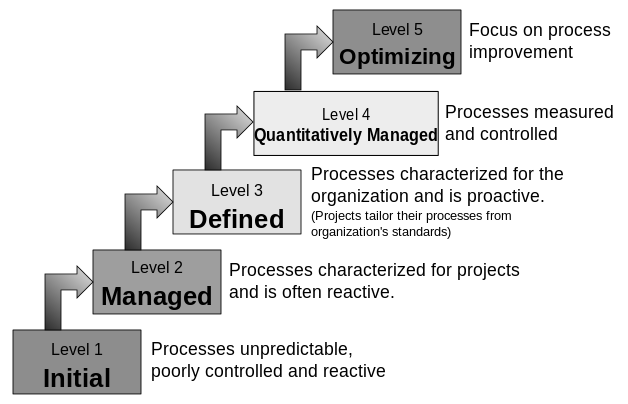
\includegraphics[scale=.7]{images/cmmi.png}
            \caption[Characteristics of CMMI]{Characteristics of CMMI, image adapted from  \cite{Godfrey} }
            \label{fig:cmmi}
        \end{figure}

A visual description of the CMMI maturity levels can be seen in Figure \ref{fig:cmmi}.  
While CMMI-Dev does provide an excellent framework for improving a process.  It
is wholely focused on process improvement.  It does not provide guidelines
for evaluating the final product.  
Also, it does not provide a specify mechanism for evaluating
or scoring the progression through the maturity levels.  
An indicator is still needed to quantify the overall performance of an organization, not
just the compliance to standard processes.  


\subsection{PREVIOUS SOFTWARE EVALUATION ATTEMPTS }

Sextant is a visualization tool for Java source code \cite{Winter2013}.  Sextant provides a graphical representation of the information related 
to a software system.  The tool provides the capability to provide custom rules which are specific to the domain or application.  However,
Sextant only provides metrics and analysis of the software code.  It provides no information regarding the rest of the 
software development lifecycle.  Also, the primary output of Sextant is visual graphs.  While these graphs do provide
useful information, they do not provide a single number to determine the performance of the software.

\textit{Software process mining} \cite{Rubin2007} provides
an algorithm and information for measuring a software engineering process from
the Software Configuration Management (SCM). Software process mining does provide a method for tracking all 
documentation that can be placed in SCM, not just source code.  The technique creates process models 
to understand the process of developing software and code. It is less focused on the output and results,
but it is more focused on conformance to a process or understanding the process. Once again, a single number is not produced.

One example of scoring software development is presented by Jones \cite{Jones2012}. The methodology looks
for the presence of various techniques used in software engineering.  The methodology provides a score based upon the 
productivity and quality increase of the technique being evaluated.  Points are positive or negative based upon the 
presense of various techniques. A couple example techniques are: 
automated source code analysis and continuous integration.  The end result is a score in range $[-10,10]$. 
While the result is a single number score, it does not account for the entirety of the software development lifecycle.

Much work has been done to determine metrics for source code, in fact 
entire books have been written on the topic of software metrics \cite{Jones1996, Putnam2013}. Yet, 
organizations still struggle to measure the production of software.
Little work exists
for scoring the entire software development organization. 

\subsubsection{SOFTWARE QUALITY}
Quality is tested in \cite{Miguel2014}

\subsubsection{SOFTWARE ANALYTICS}
What is software analytics?

Some of the measurements focus specifically on the source code; analyzing the 
complexity, size, and coupling \cite{Tosi2012}. 

Letier and Fitzgerald discuss how to choose the correct tools and techniques to analyze
software data \cite{Letier2013}.  A goal model is produced that matches the data analysis methods
with the goals of the software stakeholders.  Again, the method does not focus
on analysis of development of software.

\textit{Software Development Analytics} is a subfield of software analytics 
\cite{Menzies2012}.  It focuses on the analytics of the development of software, not
the overall performance of the software.  

Software development produces many value pieces of datum that can be analyzed
\cite{Marcus2010}. Just a few of the pieces of datum are:
email communication, bugs, fixes, source code, version control system histories,
process information, and test data.  Examples of this type of data
can be found in the PROMISE Data Repository \cite{promise12}.

See also \cite{Buse2010}.  



\subsubsection{COCOMO}  
    Constructive Cost Model (COCOMO) is a software cost estimation model created
    by Boehm \cite{Boehm1981}.  It combines future project characteristics
    with historical project data to create a regression model to estimate the 
    cost of a software project.  The original version developed in 1981 was
    focused on mainframe and batch processing.  An unpdated version, named
    COCOMO II, was created by Boehm in 1995 to be more flexible for newer 
    development practices such as desktop development, off the shelf components,
    and code reuse.  COCOMO provides a nice algorithm for making decisions
    regarding building or buying software products.  It does not provide 
    an algorithms to review past performance of estimates and modify the
    algorithm accordingly.  COCOMO II can be a useful tool for an SDO,
    but it only provides an estimate and not an evaluation of the actual
    performance.



\subsubsection{SEMAT}

    Software Engineering Method and Theory (SEMAT) is claiming to be the ``new software engineering'' 
    \cite{Jacobson2014}.  The authors rightfully claim that software engineering lacks
    an underlying theoretical foundation found in other engineering disciplines.  This lack of theory
    has led software engineering to not be engineering, but rather a craft.  The goal of 
    SEMAT is to merge the craftsmanship and engineering to provide a foundation for software
    engineering.  The primary initiative of SEMAT has been the creation of a kernel for 
    software engineering.  The kernel is the minimal set of things common to all software development
    endeavours. The three parts to the kernel are:
    \begin{description}
        \item[Measurement] - There must exist a means to determine the health and progress of an endeavour
        \item[Categorization]-  The activities must progress through categories during an endeavour
        \item[Competencies] - Specific competencies will be required for completing activities
    \end{description}
    The kernel defines alphas, which are seven dimensions with
    specific states for measuring progress. 
    The seven dimensions are: 
    \begin{enumerate}
        \item Opportunity
        \item Stakeholders
        \item Requirements
        \item Software Systems
        \item Work
        \item Team
        \item Way of Working
    \end{enumerate}
    
    Although SEMAT is very promising, the development is not yet complete.  Adoption is
    limited so the technique has not been validated on many
    actual software engineering endeavours.  Although SEMAT does include a part for
    measurement of progress, it does not specify how the measurement is to be 
    performed.
    
    So it has been shown, there exist many attempts to 
    evaluate portions of the a software development 
    organization.  None of the the attempts provide
    a single number score for the entirety of the 
    organization.  Most of the techniques focus on
    specific portions of the software development 
    lifecycle, namely the development portion. 
    
    


\subsection{ORGANIZATION OF THE WORK}

The remainder of this dissertation is divided into 5 chapters.  The next chapter provides
an overview of software, software development lifecycles, software engineering, and software
development organizations.  Chapter 3 introduces what is meant by the term data-driven
software engineering. Chapter 4 then provides an explanation of the Master Performance 
Indicator (MPI).  It will present the essential elements for calculating the MPI, as well
as the formulas, frameworks, and data necessary to produce the MPI. Chapter 5 provides
a technological framework for generating and storing the current and historical MPI values.
Chapter 6 demostrates how MPI can be implemented in a software development portion of 
a large financial institution.  Chapter 7 concludes the dissertation with a summary
of the results and some possible future directions for further enhancements. 

\end{document}